%%
%% Edward T. Norris
%% Discrete Ordinates Computed Tomography Organ Dose Simulator (DOCTORS)
%% 
%% === Implementation ===
%%

This chapter covers the details of the implementation of the different components of the DOCTORS code base.

The code is available from a GitHub Git repository. At the time of this writing, the repository is located at \texttt{https://github.com/eNorris/thesis} and is only available subject to special request and license agreement. An executable version is available.

The code is implemented in C++ and requires a C0x11 compliant compiler. The user interface is written using the Qt5 framework. GPU computation is performed via CUDA which must be compiled seperatly by Nvidia's proprietary compiler, \texttt{nvcc}.

\section{Vector Flattening}\label{sec:flatten}

Data is stored as \texttt{std::vector<>} objects.

Figure~\ref{fig:indx_ex} gives an example of the spatial indexing scheme using an $8 \times 8 \times 8$ mesh. The indicated voxel has $i_x$, $i_y$, and $i_z$ indices of 1, 5, and 6 respectively. Therefore, the index value of the highlighted voxel is $1 \times 8 \times 8 + 5 \times 8 + 6$ = 110. This flattening pattern continues to higher dimensional phase space to encompas energy and direction.

\begin{figure}[tb]
  \begin{center}
   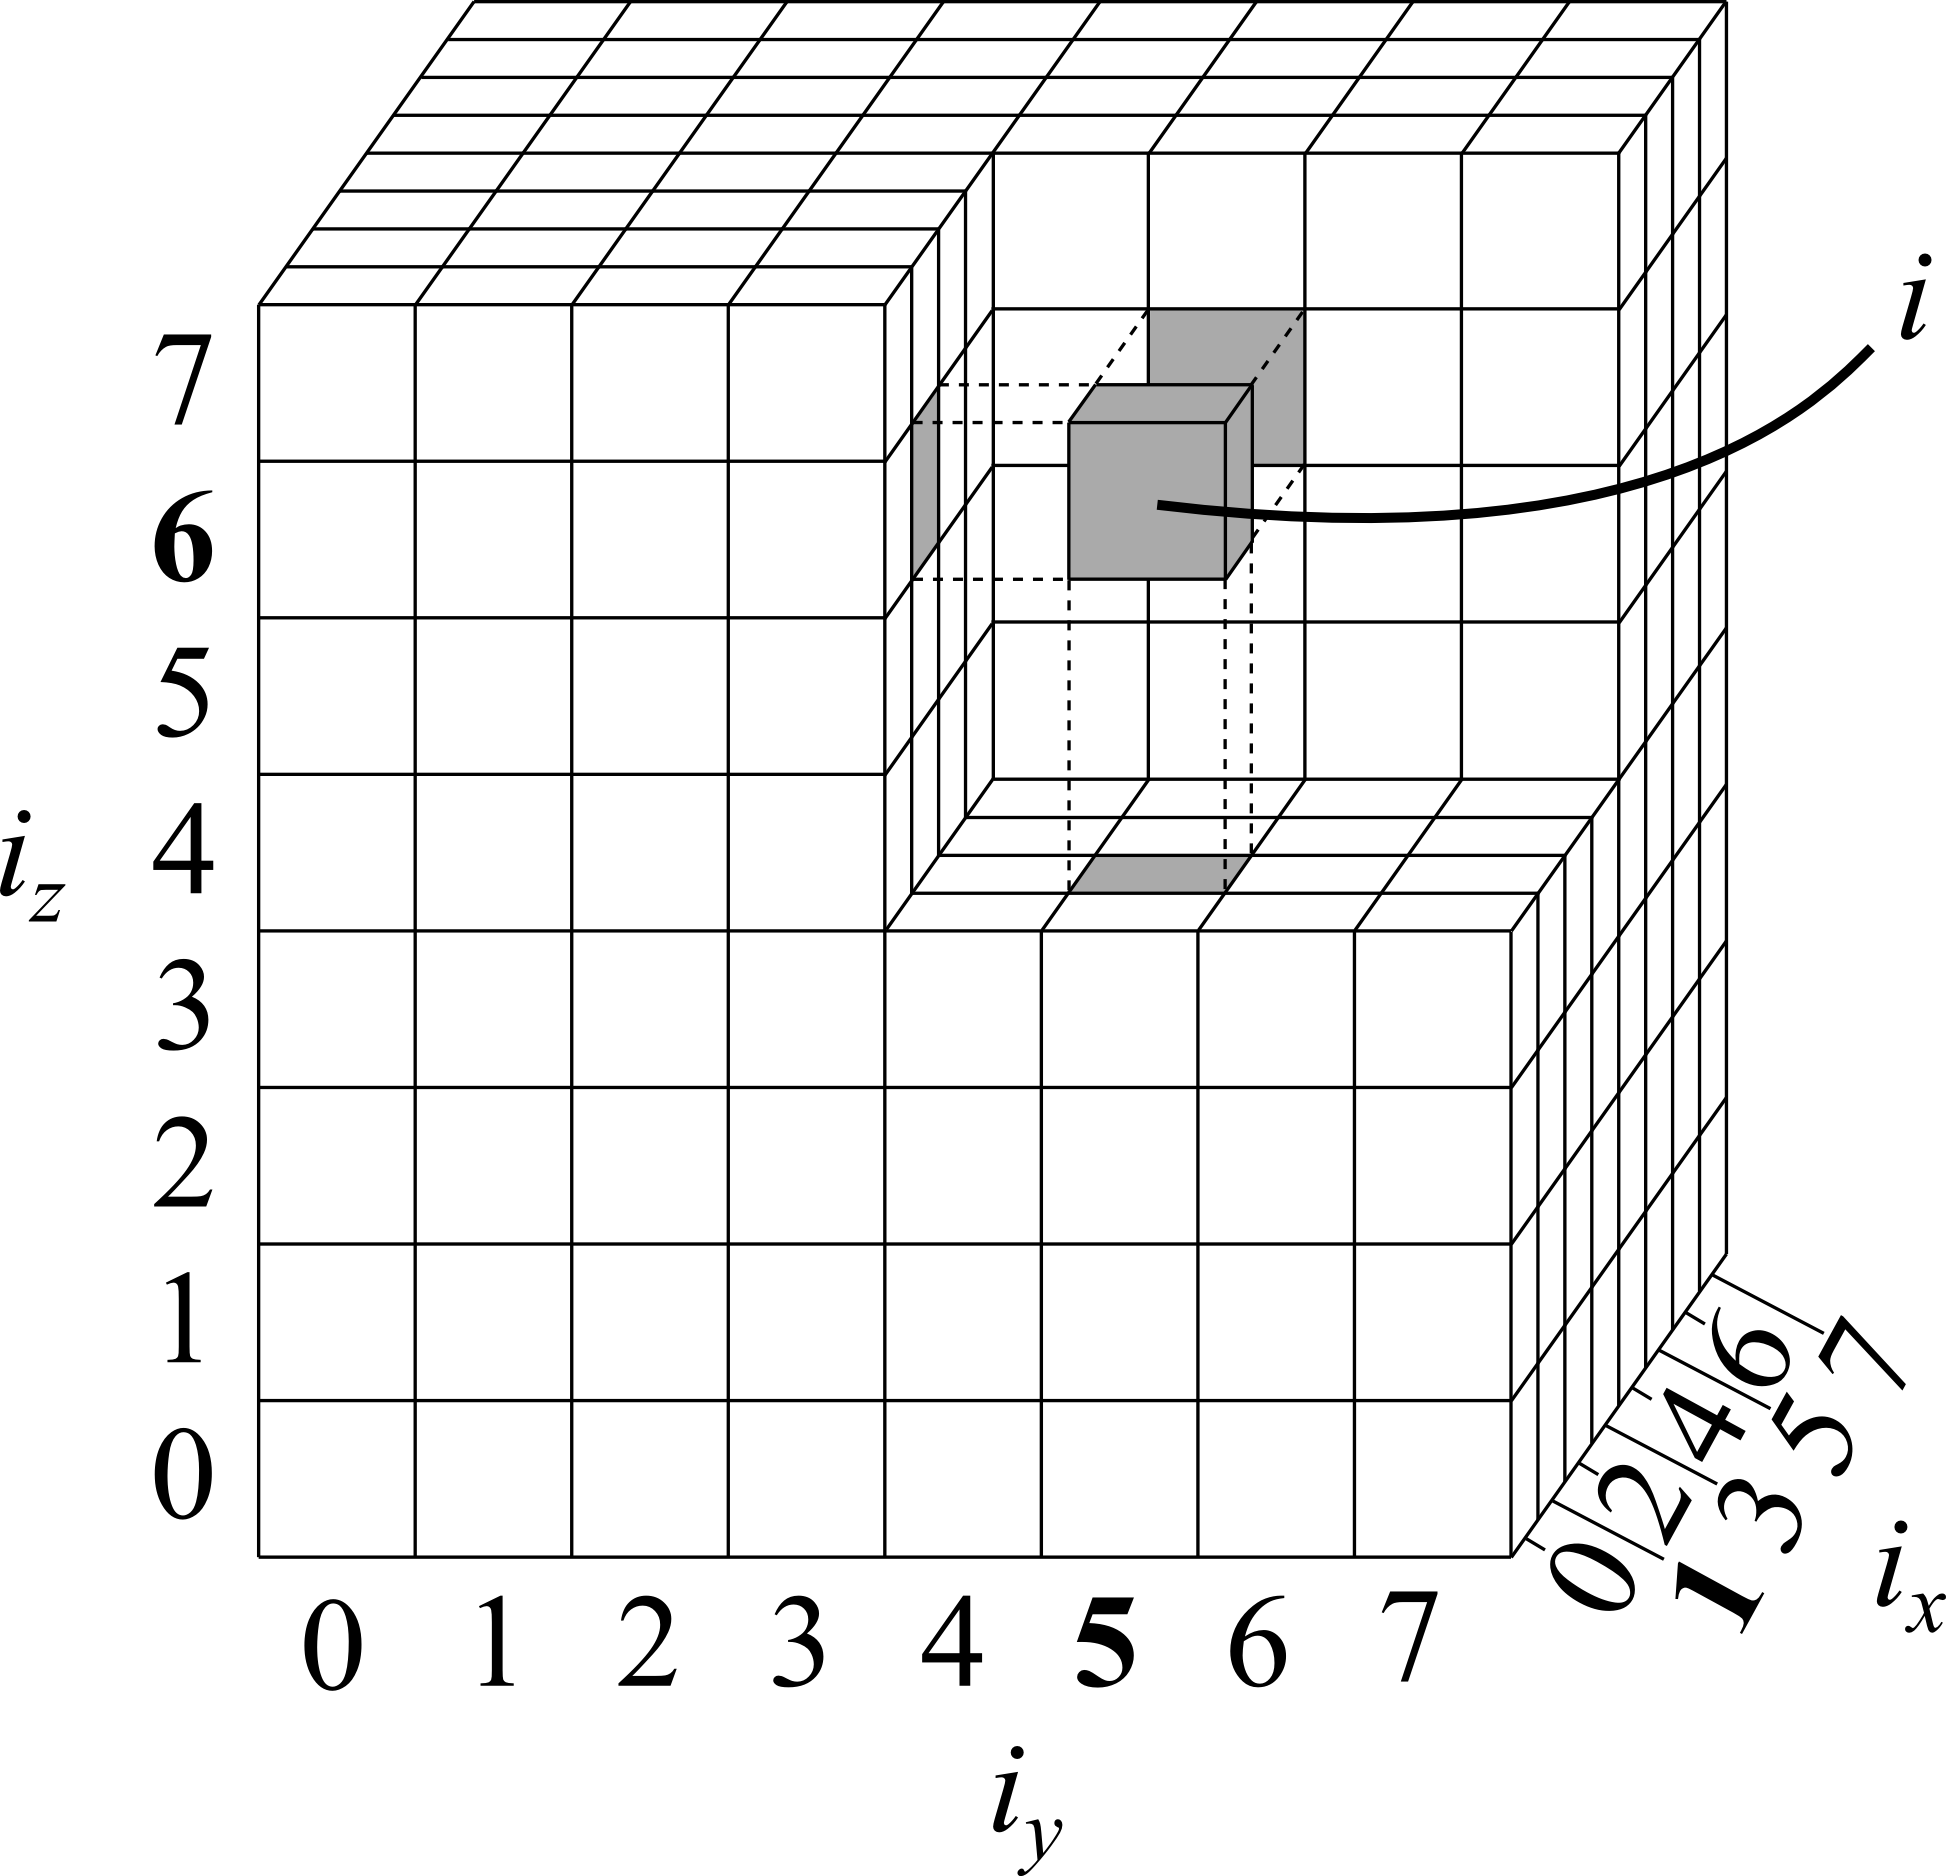
\includegraphics[width=3.75in]{figs/indx_ex}
  \end{center}
  \caption{The indexing scheme.}
\label{fig:indx_ex}
\end{figure}

A variable that is dependent on $x$, $y$, $z$, $E$, and $\Omega$ would be written as $\phi(x, y, z, E, \Omega)$ would be discretized to $\phi(i_x, i_y, i_z, G, i_a)$. Rather than storing $\phi$ as a 5-dimensional matrix, $\phi$ is stored as a 1-dimensional vector of the same number of elements.

\section{Cross Section Parsing}\label{sec:xsparse}
AMPX cross sections are stored in a binary format. The binary file is split into a series of records. Each record contains a string of binary bytes between a four byte header and four byte footer. The header and footer are identical and, when interpreted as a signed four byte integer, give the size in words of the record. Each word is a 32-bit section (4~bytes) of binary data. An example record is shown in Fig.~\ref{fig:ampxbytes1}.

The data is stored in Big Endian format which must be converted to Little Endian for most Intel and AMD processors.  The endianess rearrangement is shown in Fig.~\ref{fig:ampxbytes2}. All records are one of 12 unique types. Each type of record is formatted and interpreted differently. For example, Type 1 contains general information about the data file such as the number of nuclides, number of energy groups, and a brief description. Type 2 records contains a list of floating-point numbers representing the energy group boundaries. Figure~\ref{fig:ampxbytes1} shows a Type 1 record. In the case of the header bytes given in Fig.~\ref{fig:ampxbytes1} and~\ref{fig:ampxbytes2}, the bytes correspond to the integer 440 which is the length in bytes of the record (not including the header or footer).

Each word of data is sequentially read, reordered, and converted to an apprpriately typed variable. Table~\ref{tab:reorder} shows the converstion for the record given in Fig.~\ref{fig:ampxbytes1}.

\begin{figure}[tb]
  \begin{center}
   \includegraphics[width=3.75in]{figs/ampxbytes1}
  \end{center}
  \caption{An example record parsed. The header and footer are identical and are the number of 32-bit words in the record.}
\label{fig:ampxbytes1}
\end{figure}

\begin{figure}[tb]
  \begin{center}
   \includegraphics[width=2.75in]{figs/ampxbytes2}
  \end{center}
  \caption{The byte reordering from Big Endian to Little Endian. Individual bits withing a byte are not rearranged, but the ordering of the four bytes withing a 32-bit word is reversed.}
\label{fig:ampxbytes2}
\end{figure}

\begin{table}[ht]
\caption{Byte Reordering}
\centering 
\begin{tabular}{l | c | c | c | l}
  \hline \hline   
  Word  & Big Endian & Little Endian & Interpreted & Notes\\ [0.5ex] % inserts table 
  \hline
  0   & B8 01 00 00 & 00 00 01 B8 & 440    & Header                    \\
  1   & 8B 69 00 00 & 00 00 69 8B & 27019  & ID                        \\
  2   & A4 01 00 00 & 00 00 01 A4 & 420    & Number of nuclides        \\
  ... &      ---    &      ---    &    --- & ---                       \\
  11  & 70 75 6F 43 & 43 6F 75 70 & "Coup" & First word of the title   \\
  12  & 20 64 65 6C & 6C 65 64 20 & "led " & Second word of the title  \\
  ... &     ---     &    ---      &  ---   & ---                       \\
  440 & 20 20 20 20 & 20 20 20 20 & "    " & 4 spaces ending the title \\
  441 & B8 01 00 00 & 00 00 01 B8 & 440    & Footer                    \\ 
  [1ex]      % [1ex] adds vertical space
  \hline
\end{tabular}
\label{table:reorder}
\end{table}

The header always reports the number of 8-bit bytes required to store the data. However, some data types, such as texttt{char}, are only one byte so each word represents multiple (4 in the case of \texttt{char}) distinct characters.

DOCTORS reads AMPX fromatted binary data files. Figure~\ref{fig:ampx} shows the data format of the overall file. 

The first entry in each nuclide entry is the directory record. The directory contains general information regarding the nuclide and information necessary to parse the proceeding records. Following the directory, Bondarenko data, resonance parameters, neutron data, and gamma production which are not of interest in photon only problems are read.

The penultimate record contains the average cross section data. This data is averaged over all energies and directions using Eq.~\ref{eq:groupxs}. The only data used in this section in DOCTORS is the total cross section values necessary for implementing the fully discretized form of the LBE given in Eq.~\ref{eq:boltz_i}.

The 2D data is stored in a special format optimized for scatter matrix data.

\begin{figure}
    \centering
    \begin{subfigure}[b]{0.45\textwidth}
        \includegraphics[width=\textwidth]{figs/ampx1}
        \caption{The AMPX file format}
        \label{fig:ampx1}
    \end{subfigure}
    ~
    \begin{subfigure}[b]{0.45\textwidth}
        \includegraphics[width=\textwidth]{figs/ampx2}
        \caption{The structure of each individual record.}
        \label{fig:ampx2}
    \end{subfigure}
    \caption{The format of the AMPX file. (a) The file contains a header, a list of directory records, energy group information and a list of nuclide entries. (b) Each nuclide entry contains multiple records; the two of concern in this work are the last two containing gamma data.}\label{fig:ampx}
\end{figure}

Figure~\ref{fig:sigmacomp} shows the microscopic cross section data pulled from 

\begin{figure}
    \centering
    \begin{subfigure}[b]{0.45\textwidth}
        \includegraphics[width=\textwidth]{figs/sigmacomp1}
        \caption{}
        \label{fig:ampx1}
    \end{subfigure}
    ~
    \begin{subfigure}[b]{0.45\textwidth}
        \includegraphics[width=\textwidth]{figs/sigmacomp2}
        \caption{}
        \label{fig:ampx2}
    \end{subfigure}
    \caption{The microscopic cross section in bars for hydrogen and oxygen. Both subfigures show identical data, (a) shows the entire data range available in the reference data library and (b) shows only the data range applicable to DOCTORS.}\label{fig:sigmacomp}
\end{figure}

\section{Generation of Material Cross Section Data}\label{sec:xsgen}

Once the data is parsed, weighted combinations of elemental data is used to create material cross sections.

MT AND MF NUMBERS

WATER EXAMPLE.

\begin{figure}
    \centering
    \begin{subfigure}[b]{0.45\textwidth}
        \includegraphics[width=\textwidth]{figs/airwaterxs2_19group}
        \caption{19 group data}
        \label{fig:airwaterxs2_19group}
    \end{subfigure}
    ~
    \begin{subfigure}[b]{0.45\textwidth}
        \includegraphics[width=\textwidth]{figs/airwaterxs2_47group}
        \caption{47 group data.}
        \label{fig:airwaterxs2_47group}
    \end{subfigure}
    \caption{Comparison of the group-averaged DOCTORS cross section data to continuous NIST data.}\label{fig:airwaterxs_group}
\end{figure}

\section{Qt5 Framework}\label{sec:qt}
The Qt5 framework was used for implementation of the user interface. Qt5 enables asynchronous calls through its ssignal/slot mechanism. A signal can be emitted which will execute all connected slots. Signals and slots can be connected manually by the user except for ones automatically generated by Qt. Qt prvides a user interface for building user interfaces. Components such a sbuttons, drop boxes, radio buttons, etc. are offered to the user. Qt makes extensive use of polymorphism. All user components inherit from the base \texttt{QWidget} class which inherits from \texttt{QObject}. Any class that utilizes the signal/sloot mechanism must extend the \texttt{QOjbect} class.

Listing~\ref{lst:sync1} gives a pseudocode snippet that has a long function that will block the user interface. A corresponding dequence diagram is given in Fig.~\ref{fig:sync1}. When the user interacts with the GUI, the writer object begins executing the \texttt{doWrite()} function. Until this function completes, the UI thread will be busy an dunable to handle additionaly user interaction or updates. This results in the GUI becoming unresponsive and potentially issuing a warning to the user from the operating system.

\begin{listing}
\begin{minted}[frame=lines,linenos]{python}
import numpy as np
def myfcn(hello,world):
   return hello*world
\end{minted}
\caption{Blah blah blah.}\label{lst:sync1}
\end{listing}

\begin{figure}[tb]
  \begin{center}
   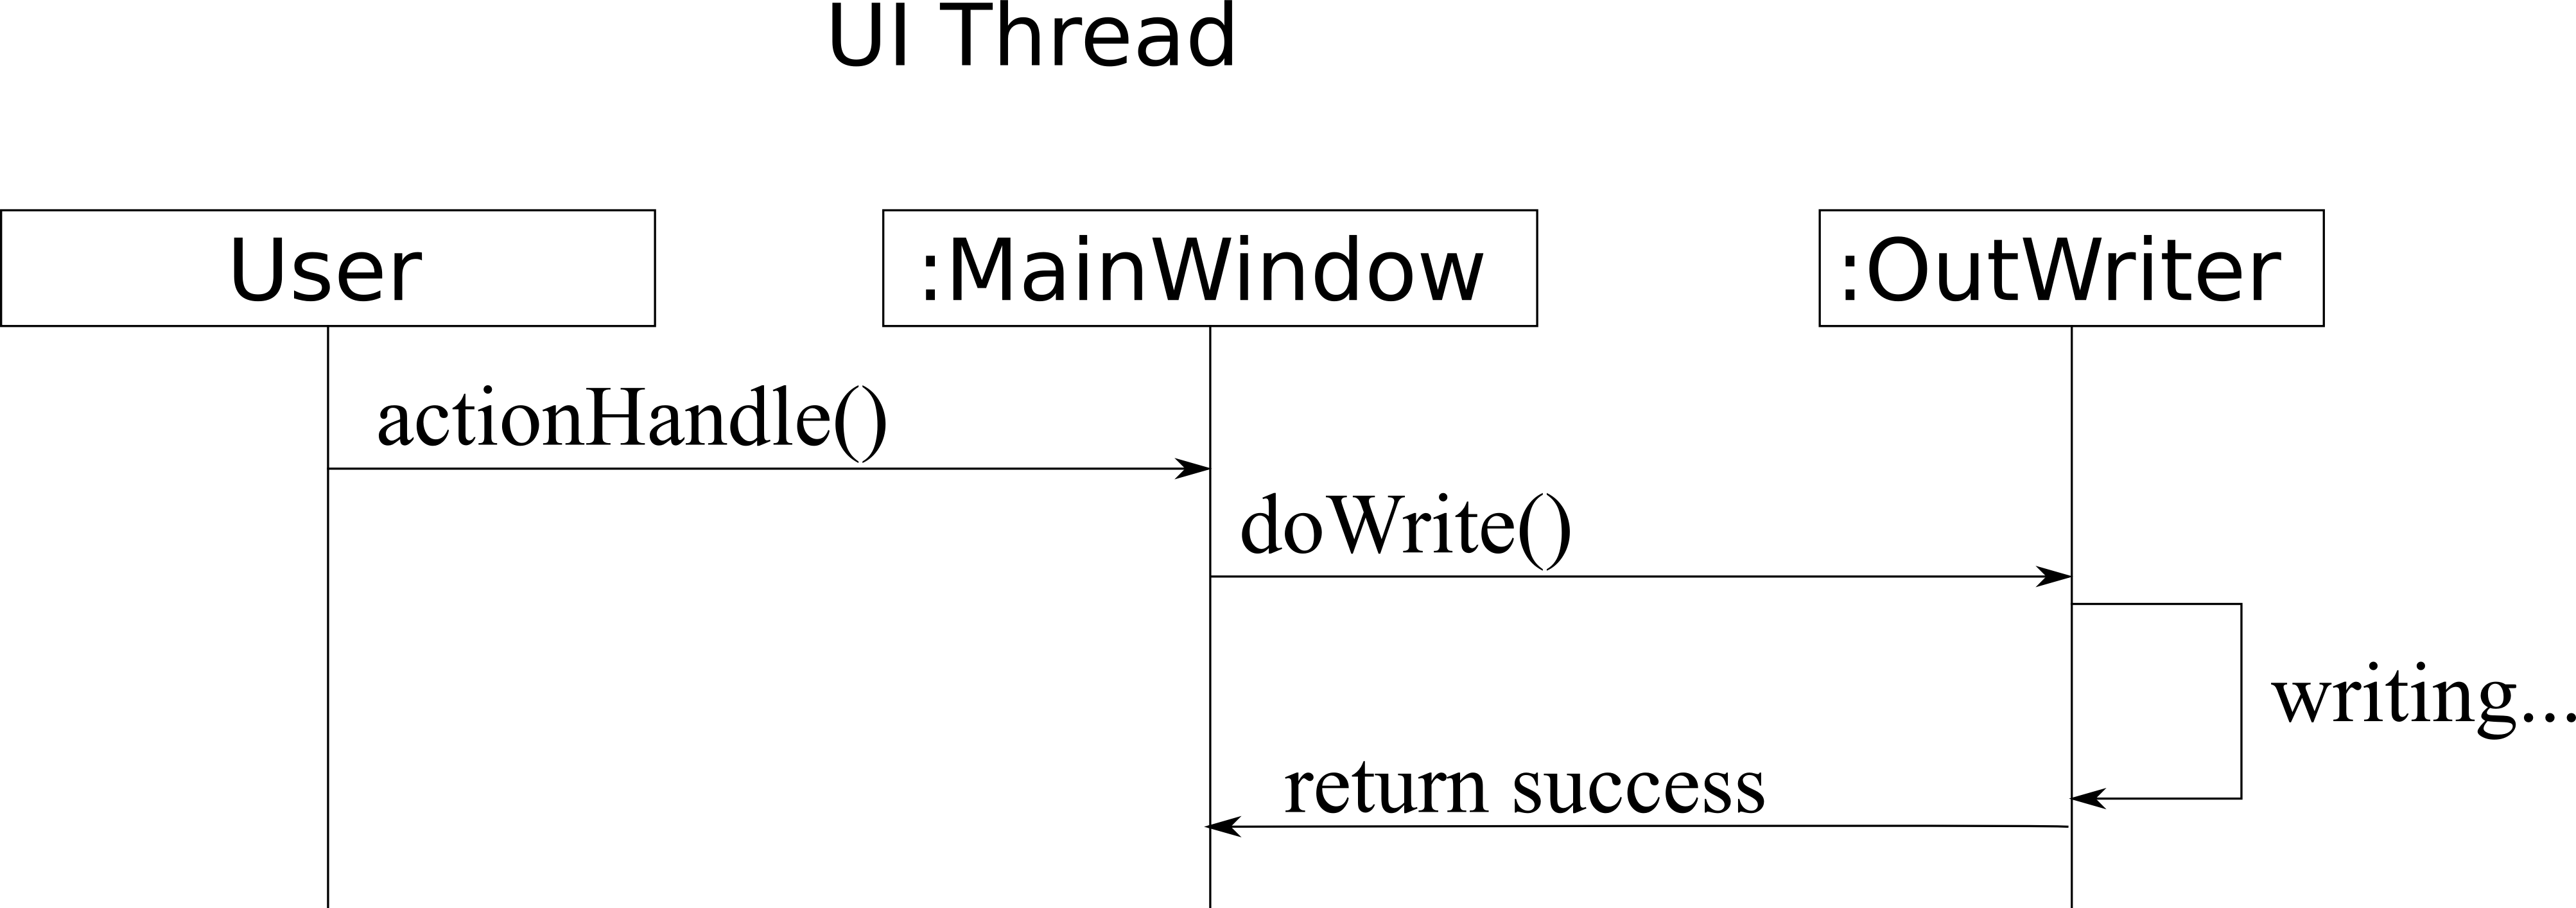
\includegraphics[width=3.75in]{figs/writer_sync}
  \end{center}
  \caption{Sequence diagram for the synchronous call.}
\label{fig:sync1}
\end{figure}%

The code in Listing~\ref{lst:sync1} is updated to use the Qt signal/slot mechanism.

\begin{figure}[tb]
  \begin{center}
   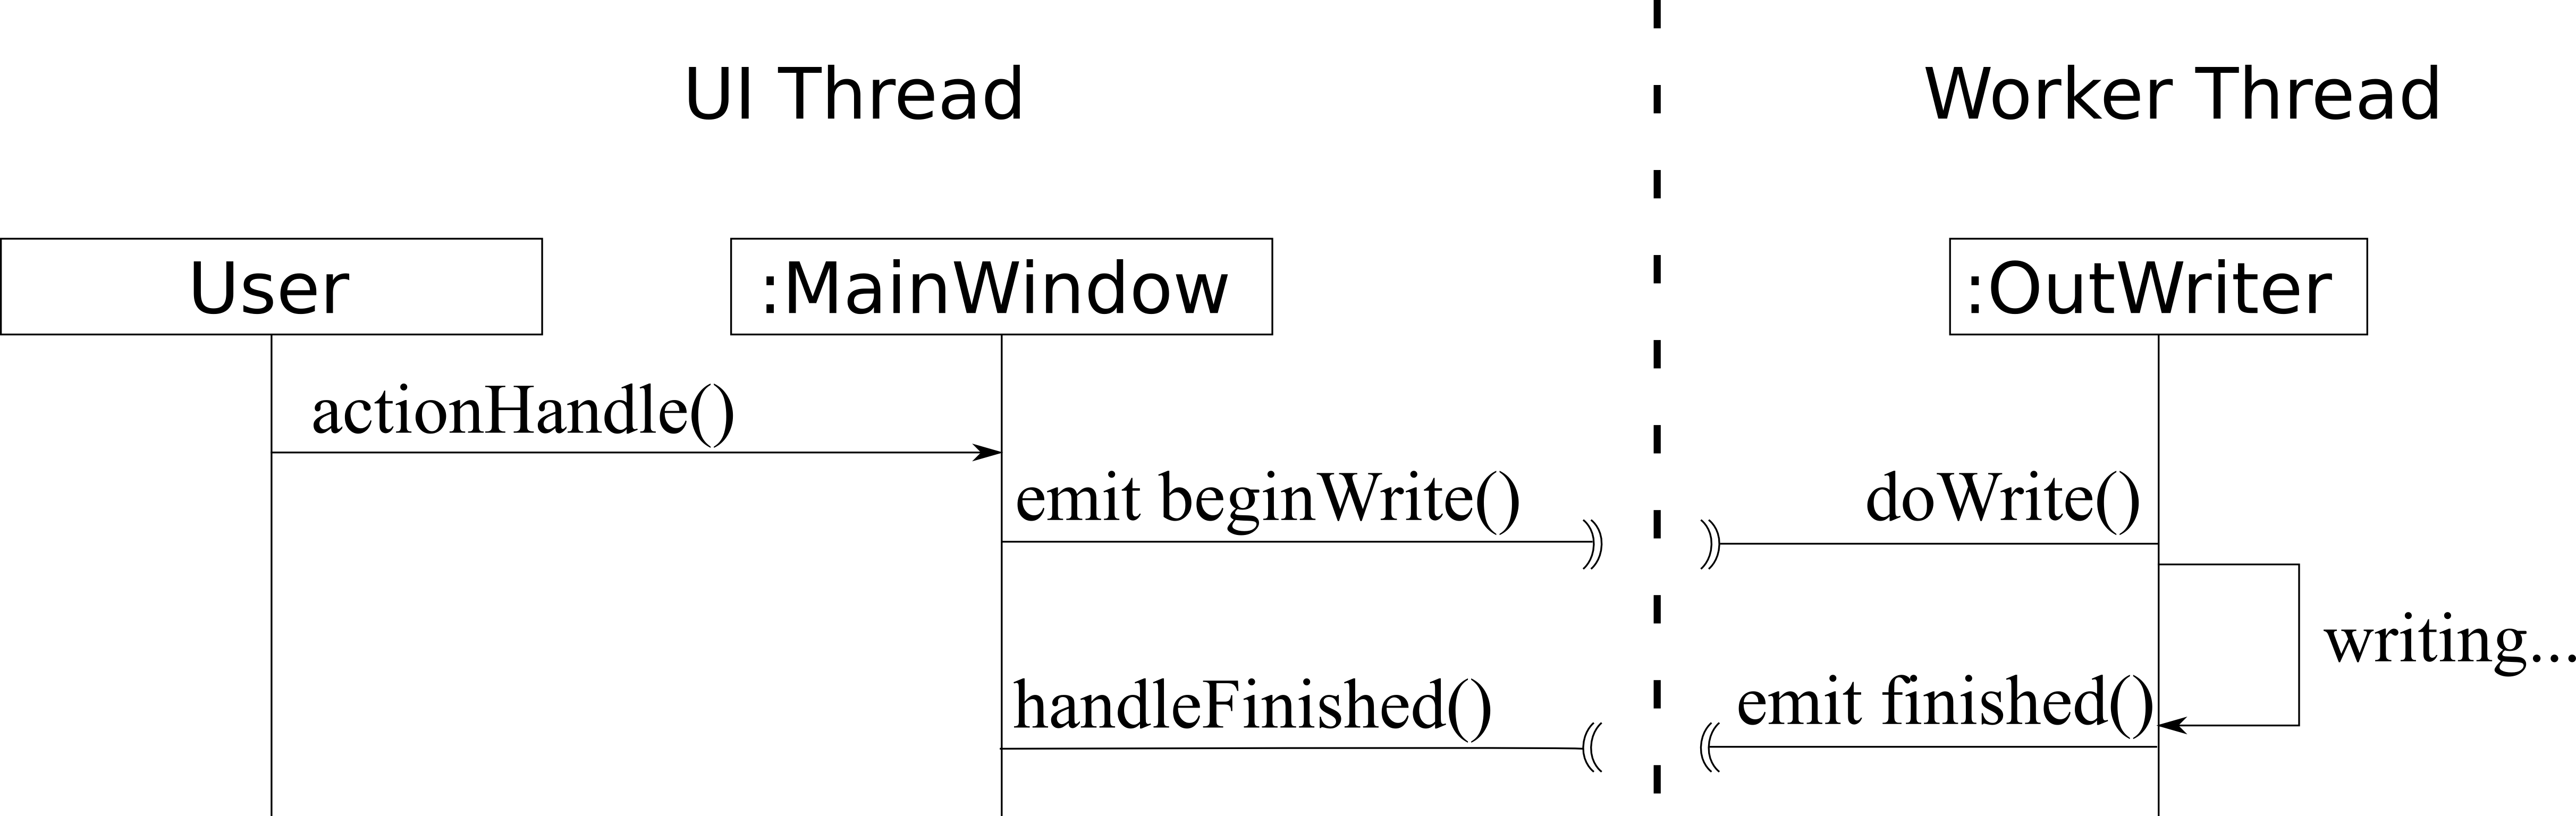
\includegraphics[width=3.75in]{figs/writer_async}
  \end{center}
  \caption{Sequence diagram for the synchronous call.}
\label{fig:async1}
\end{figure}%

\section{Graphical User Interface}\label{sec:gui}

The GUI is cool. Lots of pictures of it.

\section{CUDA}\label{sec:cuda}
CUDA code is compoiled with the Nvidia complier nvcc. Qt uses the gcc compiler and its MOC generator for meta code. In order to connect CUDA code to the Qt MOC, the CUDA code is compiled by nvcc to produce a .o file. Qt then compiles all other files into corresponding.o files. The linker than automactically picks up all of the .o files gneerated by nvcc. The final result is an executable that has a Qt generarted user interface that can communicat with an Nvidia graphics card through the CUDA language.

The sweep through the mesh is different.

\begin{table}[ht]
\caption{Subsweep Indices}
\centering 
\begin{tabular}{l | c | c | c | c}
  \hline \hline   
  i  & ix & iy & iz & ix+iy+iz \\ [0.5ex] % inserts table 
  \hline
  0  & 4 & 0 & 0 & 4\\
  1  & 3 & 1 & 0 & 4\\
  2  & 3 & 0 & 1 & 4\\
  3  & 2 & 2 & 0 & 4\\
  4  & 2 & 1 & 1 & 4\\
  5  & 2 & 0 & 2 & 4\\
  6  & 1 & 3 & 0 & 4\\
  7  & 1 & 2 & 1 & 4\\
  8  & 1 & 1 & 2 & 4\\
  9  & 1 & 0 & 3 & 4\\
  10 & 0 & 4 & 0 & 4\\
  11 & 0 & 3 & 1 & 4\\
  12 & 0 & 2 & 2 & 4\\
  13 & 0 & 1 & 3 & 4\\
  14 & 0 & 0 & 4 & 4\\ [1ex]      % [1ex] adds vertical space
  \hline
\end{tabular}
\label{table:subsweep}
\end{table}

We first split the sweep process into $N_L$ subsweeps. For a $N_x \times N_x \times N_x$ mesh, the subsweep process is straightforward. Some of the initial subsweeps are shown for a $8 \times 8 \times 8$ mesh in Fig.~\ref{fig:subsweep_cube}. This is valid for any direction, $\hat{\Omega}$, for which all three of its direction cosines ($\mu$, $\xi$, and $\eta$) are positive.

\begin{figure}
    \centering
    \begin{subfigure}[b]{0.45\textwidth}
        \includegraphics[width=\textwidth]{figs/subsweep_cube1}
        \caption{Subsweep 0 ($S=0$)}
        \label{fig:subsweep_cube1}
    \end{subfigure}
    ~ %add desired spacing between images, e. g. ~, \quad, \qquad, \hfill etc. 
      %(or a blank line to force the subfigure onto a new line)
    \begin{subfigure}[b]{0.45\textwidth}
        \includegraphics[width=\textwidth]{figs/subsweep_cube2}
        \caption{Subsweep 1 ($S=1$)}
        \label{fig:subsweep_cube2}
    \end{subfigure}
    ~ %add desired spacing between images, e. g. ~, \quad, \qquad, \hfill etc. 
    %(or a blank line to force the subfigure onto a new line)
    \begin{subfigure}[b]{0.45\textwidth}
        \includegraphics[width=\textwidth]{figs/subsweep_cube3}
        \caption{Subsweep 6 ($S=6$)}
        \label{fig:subsweep_cube3}
    \end{subfigure}
    \begin{subfigure}[b]{0.45\textwidth}
        \includegraphics[width=\textwidth]{figs/subsweep_cube4}
        \caption{Subsweep 6 ($S=6$) with labels}
        \label{fig:subsweep_cube4}
    \end{subfigure}
    \caption{The progression of subsweeps throughout a sweep. Each subsweep must complete before those after it. Each voxel within a subsweep can be solved in parallel with all others in its subsweep.}\label{fig:subsweep_cube}
\end{figure}

In general, blah blah.

\begin{figure}
    \centering
    \begin{subfigure}[b]{0.2\textwidth}
        \includegraphics[width=\textwidth]{figs/subsweep_general1}
        \caption{$S=0$}
        \label{fig:subsweep_general1}
    \end{subfigure}
    ~ %add desired spacing between images, e. g. ~, \quad, \qquad, \hfill etc. 
      %(or a blank line to force the subfigure onto a new line)
    \begin{subfigure}[b]{0.2\textwidth}
        \includegraphics[width=\textwidth]{figs/subsweep_general2}
        \caption{$S=1$}
        \label{fig:subsweep_general2}
    \end{subfigure}
    ~ %add desired spacing between images, e. g. ~, \quad, \qquad, \hfill etc. 
    %(or a blank line to force the subfigure onto a new line)
    \begin{subfigure}[b]{0.2\textwidth}
        \includegraphics[width=\textwidth]{figs/subsweep_general3}
        \caption{$S=2$}
        \label{fig:subsweep_general3}
    \end{subfigure}
    \begin{subfigure}[b]{0.2\textwidth}
        \includegraphics[width=\textwidth]{figs/subsweep_general4}
        \caption{$S=3$}
        \label{fig:subsweep_general4}
    \end{subfigure}
    
    \begin{subfigure}[b]{0.2\textwidth}
        \includegraphics[width=\textwidth]{figs/subsweep_general5}
        \caption{$S=4$}
        \label{fig:subsweep_general5}
    \end{subfigure}
    ~ %add desired spacing between images, e. g. ~, \quad, \qquad, \hfill etc. 
      %(or a blank line to force the subfigure onto a new line)
    \begin{subfigure}[b]{0.2\textwidth}
        \includegraphics[width=\textwidth]{figs/subsweep_general6}
        \caption{$S=5$}
        \label{fig:subsweep_general6}
    \end{subfigure}
    ~ %add desired spacing between images, e. g. ~, \quad, \qquad, \hfill etc. 
    %(or a blank line to force the subfigure onto a new line)
    \begin{subfigure}[b]{0.2\textwidth}
        \includegraphics[width=\textwidth]{figs/subsweep_general7}
        \caption{$S=6$}
        \label{fig:subsweep_general7}
    \end{subfigure}
    \begin{subfigure}[b]{0.2\textwidth}
        \includegraphics[width=\textwidth]{figs/subsweep_general8}
        \caption{$S=7$}
        \label{fig:subsweep_general8}
    \end{subfigure}
    
    \begin{subfigure}[b]{0.2\textwidth}
        \includegraphics[width=\textwidth]{figs/subsweep_general9}
        \caption{$S=8$}
        \label{fig:subsweep_general9}
    \end{subfigure}
    ~ %add desired spacing between images, e. g. ~, \quad, \qquad, \hfill etc. 
      %(or a blank line to force the subfigure onto a new line)
    \begin{subfigure}[b]{0.2\textwidth}
        \includegraphics[width=\textwidth]{figs/subsweep_general10}
        \caption{$S=9$}
        \label{fig:subsweep_general10}
    \end{subfigure}
    ~ %add desired spacing between images, e. g. ~, \quad, \qquad, \hfill etc. 
    %(or a blank line to force the subfigure onto a new line)
    \begin{subfigure}[b]{0.2\textwidth}
        \includegraphics[width=\textwidth]{figs/subsweep_general11}
        \caption{$S=10$}
        \label{fig:subsweep_general11}
    \end{subfigure}
    \begin{subfigure}[b]{0.2\textwidth}
        \includegraphics[width=\textwidth]{figs/subsweep_general12}
        \caption{$S=11$}
        \label{fig:subsweep_general12}
    \end{subfigure}
    
    \begin{subfigure}[b]{0.2\textwidth}
        \includegraphics[width=\textwidth]{figs/subsweep_general13}
        \caption{$S=12$}
        \label{fig:subsweep_general13}
    \end{subfigure}
    ~ %add desired spacing between images, e. g. ~, \quad, \qquad, \hfill etc. 
      %(or a blank line to force the subfigure onto a new line)
    \begin{subfigure}[b]{0.2\textwidth}
        \includegraphics[width=\textwidth]{figs/subsweep_general14}
        \caption{$S=13$}
        \label{fig:subsweep_general14}
    \end{subfigure}
    ~ %add desired spacing between images, e. g. ~, \quad, \qquad, \hfill etc. 
    %(or a blank line to force the subfigure onto a new line)
    \begin{subfigure}[b]{0.2\textwidth}
        \includegraphics[width=\textwidth]{figs/subsweep_general15}
        \caption{$S=14$}
        \label{fig:subsweep_general15}
    \end{subfigure}
    \caption{The generalized subsweep.}\label{fig:subsweep_general}
\end{figure}

The number of parallel tasks, $P$, that can be done on subsweep $S$ of an $N_x \times N_y \times N_z$ mesh is given by Eq.~\ref{eq:taskspersub}.

\begin{equation}\label{eq:taskspersub}
P = C_S - L_x - L_y - L_z + G_{xy} + G_{yz} + G_{xz}
\end{equation}

\begin{equation}
C_S = \frac{(S+1)(S+2)}{2}
\end{equation}

\begin{equation}
L_x = \frac{d_x(d_x+1)}{2}
\end{equation}

\begin{equation}
L_y = \frac{d_y(d_y+1)}{2}
\end{equation}

\begin{equation}
L_z = \frac{d_z(d_z+1)}{2}
\end{equation}

\begin{equation}
G_{xy} = \frac{d_{xy}(d_{xy}+1)}{2}
\end{equation}

\begin{equation}
G_{yz} = \frac{d_{yz}(d_{yz}+1)}{2}
\end{equation}

\begin{equation}
G_{xz} = \frac{d_{xz}(d_{xz}+1)}{2}
\end{equation}

\begin{equation}
d_x = \max(S+1-N_x, 0)
\end{equation}

\begin{equation}
d_y = \max(S+1-N_y, 0)
\end{equation}

\begin{equation}
d_z = \max(S+1-N_z, 0)
\end{equation}

\begin{equation}
d_{xy} = \max(S+1-N_x - Ny, 0)
\end{equation}

\begin{equation}
d_{yz} = \max(S+1-N_y - Nz, 0)
\end{equation}

\begin{equation}
d_{xz} = \max(S+1-N_x - Nz, 0)
\end{equation}

Each voxel in a subsweep can be computed in parallel. Mathematically, the $i^{th}$ subsweep from all directions can be computed in parallel. However, in practice, this results in a race condition on the GPU hardware.


DELETE BELOW HERE.

The number of elements before the 4$^{th}$ level is 1 + 2 + 3 = 6. This is simply the sum of all integers less than the level number given by Eq.~\ref{eq:levelsum}. This is conincidentally the index of the first element of that level. However, there is a special case of $N_0 = 1$.

\begin{equation} \label{eq:levelsum}
N_L = \sum_{i=1}^{L} = \frac{L(L+1)}{2}
\end{equation}

Given an index, $i$, the level to which it belongs can be computed by substituting $i$ for $N_L$ in Eq.~\ref{eq:levelsum} and solving for $L$. The index value is then floored.

\begin{equation} \label{eq:levelquadratic}
i = \frac{L(L+1)}{2} \rightarrow L^2 + L - 2i = 0
\end{equation}

\begin{equation} \label{eq:levelquadsol1}
L = \left \lfloor{\frac{-1 \pm \sqrt{1+8i}}{2}} \right \rfloor
\end{equation}

Since the index must be a positive value, the $\pm$ sign can be removed from Eq.~\ref{eq:levelquadsol1} yielding Eq.~\ref{eq:levelquadsol2}

\begin{equation} \label{eq:levelquadsol2}
L = \left \lfloor{\frac{-1 + \sqrt{1+8i}}{2}} \right \rfloor
\end{equation}

The maximum index of any level in a the $N$ subsweep is $N$. Each subsweep adds an additional level. Therefore, the ix, iy, and iz indices can be computed using Eq.~\ref{eq:levelix},~\ref{eq:leveliy}, and~\ref{eq:leveliz} respectively.

\begin{equation} \label{eq:levelix}
ix = N - N_L
\end{equation}

\begin{equation} \label{eq:leveliy}
iy = L + N_L - i
\end{equation}

\begin{equation} \label{eq:leveliz}
iz = L + i - N_L
\end{equation}

\section{MCNP Generation}\label{sec:mcnpgen}
DOCTORS has the capability to generate MCNP6 input files from the CT mesh data and source specification provided by the user.

\section{Hardware}\label{sec:hardware}
For this work, a computer with an Intel i7-5960X 8 core (16 hyperthreads) processor with a base clock speed of 3.X GHz and an Nvidia Titan Z graphics card was used. Currently, if the problem requires more memory than is available on the GPU, the problem can still be solved, but much more time will be required to to copy overhead between the CPU and GPU. If the problem requires more memory than either the GPU or CPU can provide, an error is thrown and the simulation is not run.

CUDA is Nvidia only so AMD is not considered.

\endinput
%%
%% End of file `chapall.tex'.
